% flashcards-title: One ten exchanged for ten ones
% flashcards-desc: The quantity forty-two appears as four tens and two ones above and as three tens and twelve ones below.
\documentclass[dvisvgm,tikz,border=8pt]{standalone}
\usetikzlibrary{arrows.meta,patterns}

\definecolor{qraNavy}{HTML}{17324D}
\definecolor{qraBlue}{HTML}{2B6CB0}
\definecolor{qraGold}{HTML}{B7791F}
\definecolor{qraPale}{HTML}{EAF2F8}
\definecolor{qraGray}{HTML}{5C6773}

\tikzset{
  qra axis/.style={draw=qraNavy, line width=1.2pt},
  qra tick/.style={draw=qraNavy, line width=1pt},
  qra guide/.style={draw=qraGray, densely dashed, line width=0.8pt},
  qra counter/.style={circle, draw=qraNavy, fill=qraPale, line width=0.9pt, minimum size=7mm, inner sep=0pt},
  qra label/.style={font=\sffamily\bfseries, text=qraNavy},
  qra small label/.style={font=\sffamily, text=qraNavy},
}

\begin{document}
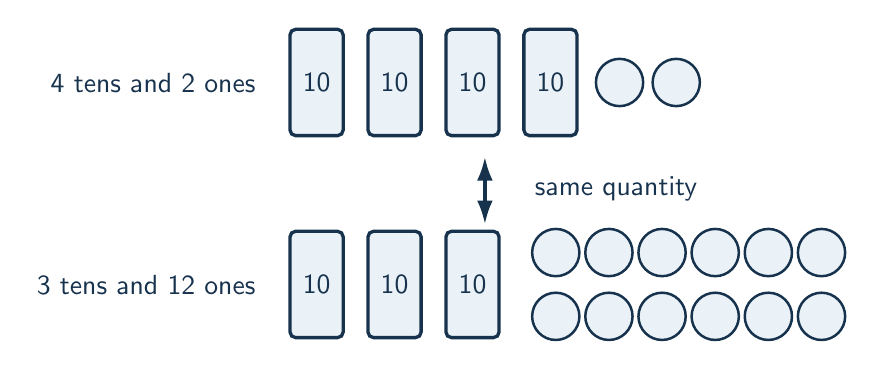
\begin{tikzpicture}[x=0.9cm,y=0.9cm]
  \node[qra small label, anchor=east] at (-0.35,2.2) {4 tens and 2 ones};
  \foreach \x in {0,1.1,2.2,3.3} {
    \draw[qra axis, rounded corners=2pt, fill=qraPale] (\x,1.45) rectangle +(0.75,1.5);
    \node[qra small label] at (\x+0.375,2.2) {10};
  }
  \foreach \x in {4.65,5.45} {
    \node[qra counter, minimum size=6mm] at (\x,2.2) {};
  }

  \draw[qra axis, {Latex[length=3mm,width=2mm]}-{Latex[length=3mm,width=2mm]}] (2.75,1.15) -- (2.75,0.2);
  \node[qra small label] at (4.6,0.7) {same quantity};

  \node[qra small label, anchor=east] at (-0.35,-0.65) {3 tens and 12 ones};
  \foreach \x in {0,1.1,2.2} {
    \draw[qra axis, rounded corners=2pt, fill=qraPale] (\x,-1.4) rectangle +(0.75,1.5);
    \node[qra small label] at (\x+0.375,-0.65) {10};
  }
  \foreach \x/\y in {3.75/-0.2,4.5/-0.2,5.25/-0.2,6/-0.2,6.75/-0.2,7.5/-0.2,3.75/-1.1,4.5/-1.1,5.25/-1.1,6/-1.1,6.75/-1.1,7.5/-1.1} {
    \node[qra counter, minimum size=6mm] at (\x,\y) {};
  }
\end{tikzpicture}
\end{document}
